A partir del montaje experimental descrito y utilizando la herramienta
\emph{Tracker Video}, se obtuvo una serie de datos de posición en función del
tiempo, como se
muestra en la \cref{fig:position}.
Cada gráfica corresponde a una gota diferente, y en ellas se observan los
instantes de ascenso y descenso.
La pendiente de cada gráfica revela las diferentes velocidades, lo cual se
atribuye a las variaciones en la masa y la carga total de cada gota.

\begin{figure*}[t]
	\centering
	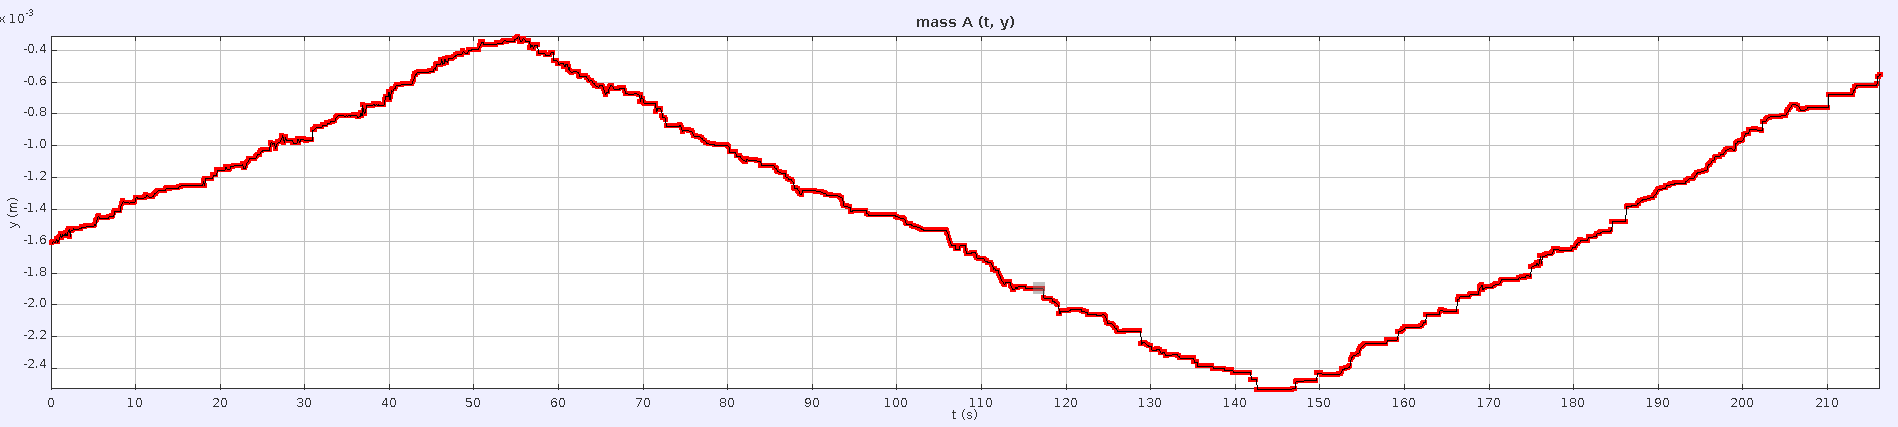
\includegraphics[width=0.8\linewidth]{./images/positon-drop-tracker-00.png}
	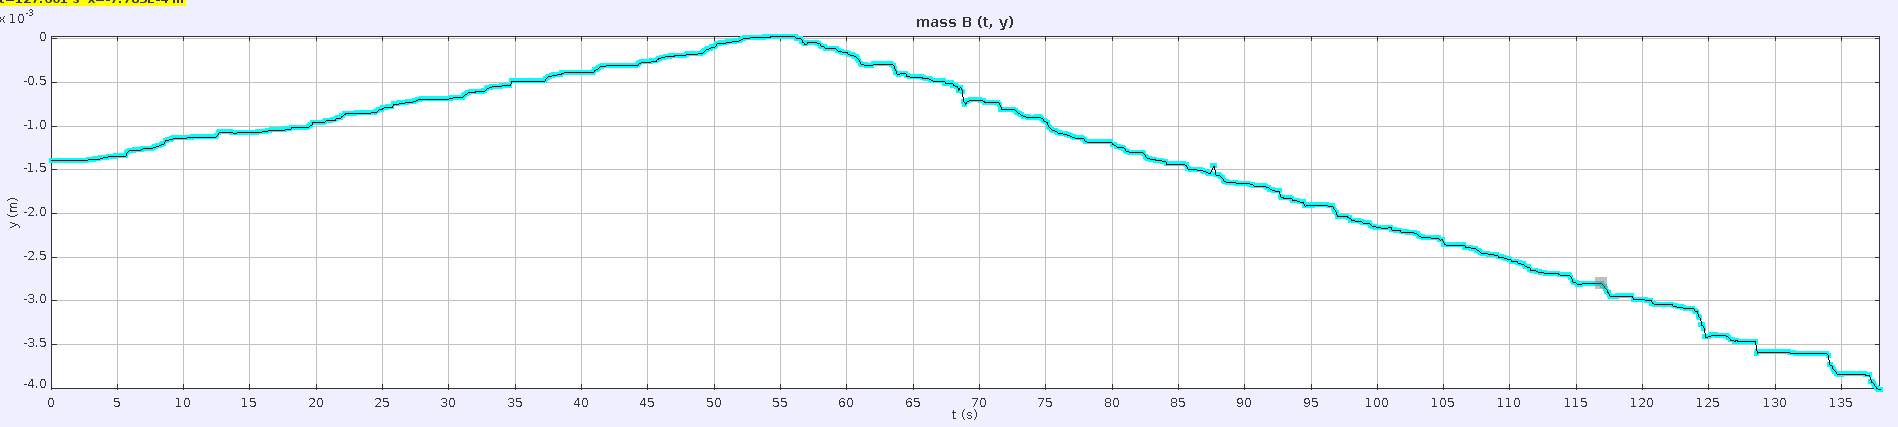
\includegraphics[width=0.8\linewidth]{./images/positon-drop-tracker-01.png}
	\caption{Posiciones a lo largo del tiempo, obtenidas con \emph{Tracker Video}.}
	\label{fig:position}
\end{figure*}

Tomando el intervalo de tiempo entre los puntos de altura máxima y mínima en
cada ciclo de subida y bajada, se calculó la velocidad media mediante el método
de diferencias finitas.
Este cálculo asume que la velocidad es constante durante el trayecto, lo cual,
aunque no es estrictamente cierto, las gráficas sugieren que se aproxima a
dicha condición.

Al realizar el análisis en \emph{Tracker Video} para un total de 20 gotas,
las velocidades obtenidas se presentan en la \cref{tab:data-drops}.
En esta tabla, además, se muestran los valores calculados para el radio y la
carga de cada gota, según las \cref{eq:radius,eq:charge}.

\begin{table*}[t]
	\centering
	\rowcolors{2}{white}{gray!25}
	\begin{tabular}{S[table-format=2.0(1)]|S[table-format=1.2e-1]|S[table-format=1.2e-1]|S[table-format=1.2e-1]|S[table-format=1.2e-2]}
		\toprule
		{$U \, (\unit{V})$} & {$v_c \, (\unit{ms^{-1}})$} & {$v_a \, (\unit{ms^{-1}})$} &
			{$r \, (\unit{m})$} & {$q \, (\unit{C})$} \\
		\midrule
		100 (1) & 1.20E-4 & 1.94E-4 & 1.04E-6 & 2.24E-17 \\
		100 (1) & 5.98E-5 & 3.85E-4 & 7.37E-7 & 2.25E-17 \\
		100 (1) & 4.87E-5 & 1.51E-4 & 6.65E-7 & 9.11E-18 \\
		100 (1) & 5.63E-5 & 4.21E-4 & 7.15E-7 & 2.34E-17 \\
		100 (1) & 4.39E-5 & 1.69E-4 & 6.32E-7 & 9.23E-18 \\
		150 (1) & 4.03E-4 & 1.29E-4 & 1.91E-6 & 4.65E-17 \\
		150 (1) & 6.41E-4 & 1.95E-4 & 2.41E-6 & 9.22E-17 \\
		150 (1) & 4.99E-4 & 6.06E-4 & 2.13E-6 & 1.08E-16 \\
		150 (1) & 1.95E-3 & 1.21E-3 & 4.21E-6 & 6.09E-16 \\
		150 (1) & 7.90E-4 & 9.00E-4 & 2.68E-6 & 2.07E-16 \\
		200 (1) & 8.00E-4 & 9.08E-4 & 2.70E-6 & 1.58E-16 \\
		200 (1) & 4.94E-4 & 6.02E-4 & 2.12E-6 & 7.97E-17 \\
		200 (1) & 1.90E-4 & 3.10E-4 & 1.31E-6 & 2.25E-17 \\
		200 (1) & 4.90E-4 & 6.00E-4 & 2.11E-6 & 7.89E-17 \\
		200 (1) & 7.85E-4 & 8.70E-4 & 2.67E-6 & 1.52E-16 \\
		300 (1) & 7.85E-4 & 8.93E-4 & 2.67E-6 & 1.02E-16 \\
		300 (1) & 7.95E-4 & 9.03E-4 & 2.69E-6 & 1.04E-16 \\
		300 (1) & 1.92E-4 & 3.00E-4 & 1.32E-6 & 1.49E-17 \\
		300 (1) & 4.94E-4 & 6.02E-4 & 2.12E-6 & 5.31E-17 \\
		300 (1) & 7.95E-4 & 8.93E-4 & 2.69E-6 & 1.04E-16 \\
		\bottomrule
	\end{tabular}
	\caption{Tabla de valores medidos para cada gota.}
	\label{tab:data-drops}
\end{table*}

A partir de los valores obtenidos para los radios y las cargas, se observa que
la mayoría de los radios se encuentran en el orden de los micrómetros.
Esto se debe a que gotas más pequeñas no pudieron ser medidas con la resolución
de la cámara y el microscopio utilizados, mientras que gotas de mayor tamaño no
mostraron una velocidad de ascenso significativa.

En cuanto a la carga, la mayoría de los valores oscila entre \(10^{-16}\) y
\(10^{-17}\) coulombs, lo que indica que las gotas estudiadas presentaron un
grado de ionización similar.
La \cref{fig:plot-radius-charge} presenta gráficamente la relación entre la
carga y el radio, excluyendo un valor atípico para facilitar la visualización
de los datos.
Basándonos en el trabajo de Millikan, es posible apreciar cómo los datos se
agrupan en niveles discretos o líneas de valor constante, una tendencia que
sería más clara con un número mayor de datos.

\begin{figure}[H]
	\centering
	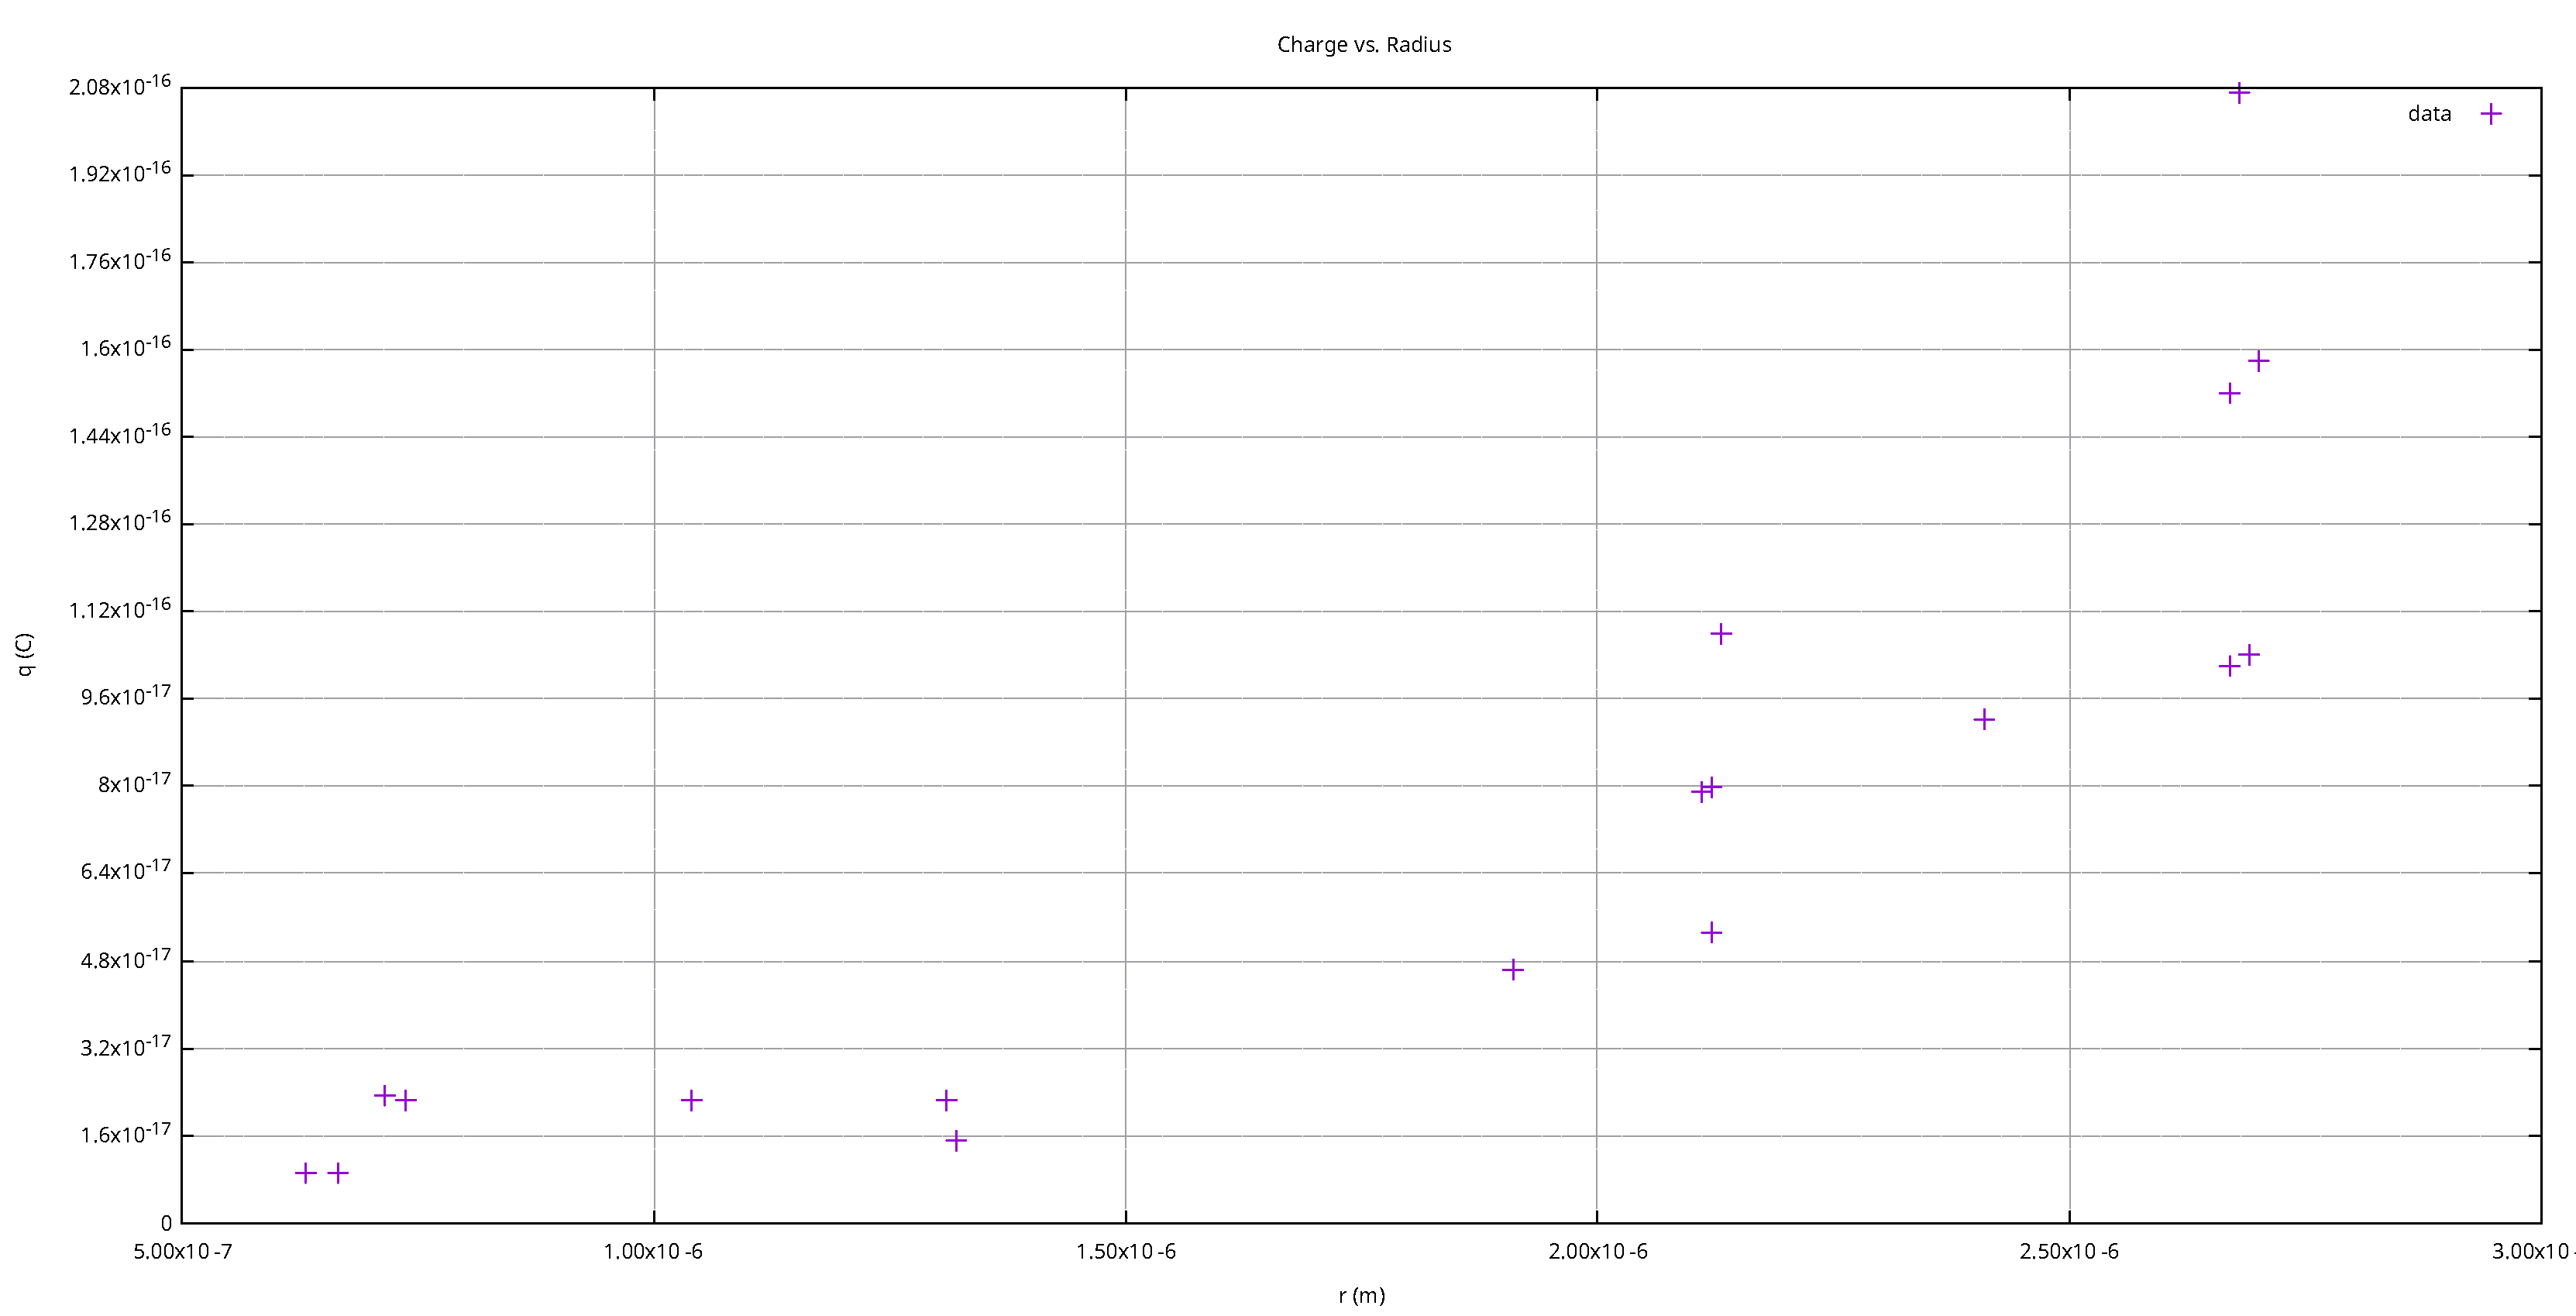
\includegraphics[width=\linewidth]{./images/plot-radius-charge.pdf}
	\caption{Carga con respecto radio de la gota.}
	\label{fig:plot-radius-charge}
\end{figure}


Dado que la carga eléctrica está cuantizada, se utilizó un código en Julia que
implementa el algoritmo euclidiano para determinar el mínimo común divisor,
excluyendo el valor de 1, con el fin de estimar el valor de \(e^{-}\).
El código arroja un mínimo común divisor de \num{1.54e-33}; el orden de magnitud
se puede omitir, ya que, según las mediciones, debería ser cercano a \(10^{-18}\).
Por lo tanto, se estima que el valor de la carga fundamental, de acuerdo con
los datos obtenidos y el análisis correspondiente, es:
\begin{equation}
	e^- \approx \qty{1.50e-19}{C}
\end{equation}

El valor obtenido presenta una discrepancia relativa del \qty{6.37}{\percent} respecto
al valor aceptado en la literatura \(e^{-} = \qty{1.602e-19}{C}\).
Esta discrepancia puede deberse a diversas suposiciones en el experimento, como
asumir que las densidades del aire y el aceite son constantes, al error numérico
introducido por el código computacional utilizado, y a la incertidumbre generada
al discretizar la posición en píxeles mediante el uso de \emph{Tracker Video}.
